\chapter{Extração de dados da WEB}
Este capítulo descreve como os dados institucionais necessários para que o MeForma2 pudesse ser utilizado pelos estudantes da Universidade Federal da Bahia (UFBA) foram obtidos. O primeiro passo para que a obtenção de dados pudesse ocorrer foi definir quais dados eram relevantes para o bom funcionamento do MeForma2. Os dados foram selecionados de acordo com as funcionalidades já existentes na primeira versão do MeForma e com as novas funcionalidades que seriam agregadas ao sistema. A Tabela~\ref{data} exibe a relação de dados que foram selecionados para a extração.

\begin{table}[H]
\begin{center}
\caption{Relação de dados extraídos da WEB para o MeForma2.}
\begin{tabular}{ |p{6cm}|p{8cm}| }
\hline
 \textbf{Dado} & \textbf{Justificativa} \\ 
 \hline
 Código de Curso & Identificar unicamente um curso na universidade. \\
 \hline
 Nome de Curso & Facilitar a identificação de um curso pelos usuários. \\
 \hline
 Código dos currículos de cada curso & Permitir a inserção de múltiplos currículos de curso no sistema. \\
 \hline
 Duração máxima e mínima de um currículo & Determinar se um usuário está atrasado com relação ao término do curso. \\
 \hline
 Carga horária obrigatória, complementar e livre de um curso & Estabelecer limites para o cálculo de completude de curso.\\
 \hline
 Código das disciplinas de um currículo & Identificar unicamente uma disciplina. \\
 \hline
 Nome das disciplinas & Facilitar a identificação de uma disciplina pelos usuários. \\
 \hline
 Carga horária de cada disciplina & Estabelecer limites para o controle de faltas e contribuir para o cálculo de conclusão de curso. \\
 \hline
 Tipo no qual uma disciplina se enquadra para cada currículo & Identificar disciplinas obrigatórias e optativas para um currículo. \\
 \hline
 Semestre recomendado para cursar uma disciplina (para as obrigatórias) & Facilitar a identificação de uma disciplina pelos usuários. \\
 \hline
 Código dos pré-requisitos de uma disciplina & Permitir estabelecer relação de dependência entre disciplinas de um currículo. \\
 \hline
\end{tabular}
\end{center}
\label{data}
\end{table}

O segundo passo foi determinar as páginas que seriam utilizadas como fonte dos dados. Esse foi um processo manual de busca por informação nos sites da UFBA, onde foram encontrados dois grupos de endereço relevantes para o processo de extração, todos pertencentes ao sistema ``Aluno Web UFBA'':

\begin{itemize}
    \item Lista de cursos da UFBA: \\
    https://alunoweb.ufba.br/SiacWWW/ListaCursosEmentaPublico.do
    \item Detalhes sobre um currículo de curso: \\
    https://alunoweb.ufba.br/SiacWWW/CurriculoCursoGradePublico.do
\end{itemize}

O primeiro grupo corresponde aos tipos de curso da UFBA, o qual espera um argumento "cdGrauCurso" que determina o tipo de curso desejado, no caso do MeForma2, só é interessante a lista de cursos de graduação. Para tal, o ``cdGrauCurso'' precisa ser ``01'':

\url{https://alunoweb.ufba.br/SiacWWW/ListaCursosEmentaPublico.do?cdGrauCurso=01}.

A Figura~\ref{cursos} exibe um fragmento da página de listagem dos cursos de graduação da UFBA. Os cursos são representados na página pelo código do cursos, e nome do curso.

\begin{figure}[H]
	   \centering
	   		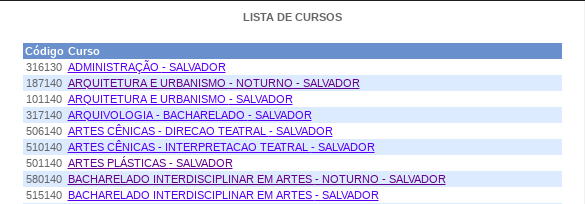
\includegraphics[scale=0.75]{pics/c4/0-cursos.png}
	   \caption{Página com listagem de cursos de graduação da UFBA.}
	   \label{cursos}
\end{figure}
O segundo grupo de endereços encontrado durante a busca manual corresponde a informações refrentes a currículos de curso e espera dois argumentos: ``cdCurso''\footnote{curiosidade: 112140 é o código identificador do curso de ciência da computação na UFBA}, que representa  o código identificador do curso de graduação em questão e ``PerCursoInicial'', que representa o currículo daquele curso. O endereço para o curso de Ciência da Computação da UFBA com o curriculo 2013.2 é:

\url{https://alunoweb.ufba.br/SiacWWW/CurriculoCursoGradePublico.do?cdCurso=112140&nuPerCursoInicial=20132}

A Figura \ref{ementa} exibe a página de detalhes de um currículo, da qual é possível obter as durações mínima e máxima de um currículo, o código do currículo e os diferentes tipos de carga horária. 

\begin{figure}[H]
    \centering
    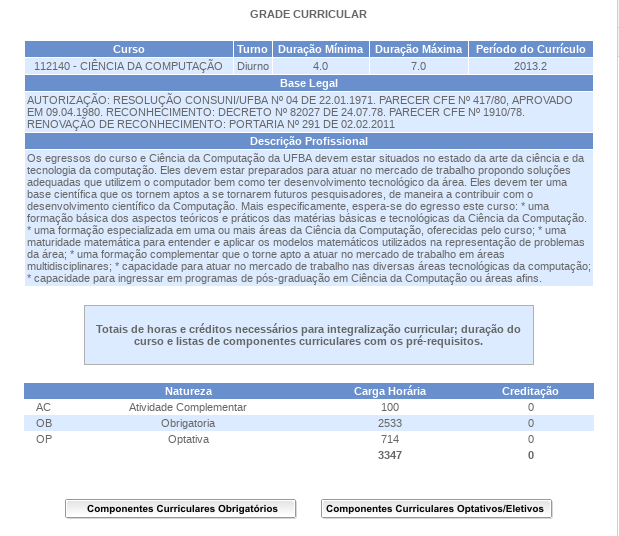
\includegraphics[scale=0.75]{pics/c4/1-ementa.png}
    \caption{Página de detalhes sobre o currículo de um curso.}
    \label{ementa}
\end{figure}

Nessa página de detalhes do currículo (Figura~\ref{ementa}) é possível encontrar dois links que precisam ser acessados através dessa página. Os links correspondem às listagens de disciplinas obrigatórias e disciplinas optativas. A lista de disciplinas obrigatórias agrupa as disciplinas por semestre. Cada disciplina de ambas as listas é representada pelo código única de disciplina, nome da disciplina e é acompanhada por sua natureza e os códigos de seus pré-requisitos, como mostra a Figura~\ref{requireds}.

Após a seleção das páginas fonte, iniciou-se a construção de um sistema de extração de dados da web focado em resolver as necessidades do MeForma2. Esse tipo de sistema é conhecido como Sistema de Web Scraping. O Web Scraping envolve o processo de consultar uma origem, recuperar a página de resultados e analisar a página para obter os resultados \cite{salerno2006method}.

O sistema de web scraping do MeForma2, apelidado de CMF, trabalha em duas etapas que se intercalam durante a recuperação de dados. As etapas correspondem aos sistemas de Web Crawler e Web Wrapper.

\begin{figure}[H]
    \centering
    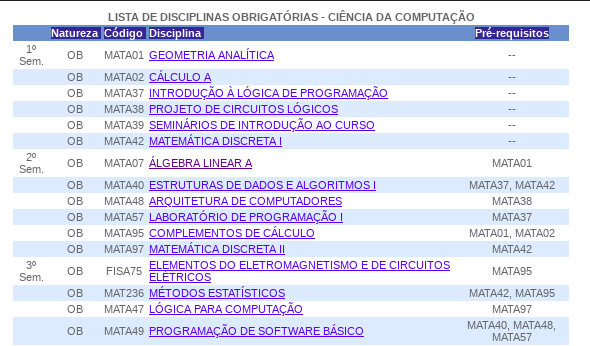
\includegraphics[scale=0.75]{pics/c4/2-requireds.png}
    \caption{Página com listagem de disciplinas obrigatórias.}
    \label{requireds}
\end{figure}

\section{Web Crawler}

Um \textit{Web Crawler}, ou simplesmente \textit{crawler}, é um programa que percorre automaticamente a estrutura de hiperlink da Web e faz o download de cada página vinculada para um armazenamento local \cite{liu}. Quando utilizado para fins de extração de dados, o \textit{crawler} deve identificar e guardar as páginas que contém os dados procurados para futura extração.

A problemática encontrada no desenvolvimento do \textit{crawler} para o MeForma2 foi que as páginas fonte não estavam conectadas. Os links das páginas de currículos não são alcançáveis a partir da página de listagem de cursos e, para acessar uma página de currículos, é necessário saber qual currículo se quer acessar e qual o código do curso referente ao currículo, informações difíceis de se obter manualmente. Contudo, a página de listagem de cursos possui, para cada curso, um endereço para uma lista de disciplinas do curso (sem seus pré-requisitos) que possui um padrão similar ao endereço fonte dos detalhes de um curso:

\url{https://alunoweb.ufba.br/SiacWWW/ListaDisciplinasEmentaPublico.do?cdCurso=316130\&nuPerCursoInicial=20111}.

Visto que o grupo de endereços encontrado na página de lista de cursos contém os parâmetros necessários para carregar a página de detalhes de um currículo, tudo o que o sistema precisou fazer foi, ao alcançar um endereço desse grupo, substituir a expressão ``ListaDisciplinasEmentaPublico'' pela expressão ``CurriculoCursoGradePublico'' antes de navegar no endereço.

\section{Web Wrapper}
O \textit{web wrapper} é um sistema de extração de dados de uma página web. O objetivo de um sistema de \textit{web wrapper}, ou simplesmente \textit{wrapper} é encontrar os dados dentro da estrutura de uma página, extraí-los, estruturá-los (conforme a finalidade para a qual está sendo executado), e exportá-los para uso futuro. De acordo com \cite{liu}, um \textit{wrapper} pode utilizar três diferentes abordagens:
\begin{itemize}
    \item Abordagem manual: Ao observar uma página da \textit{Web} e seu código-fonte, o programador humano localiza alguns padrões e, em seguida, grava um programa para extrair os dados de destino.
    \item \textit{Wrapper induction}: Nessa abordagem, um conjunto de regras de extração é aprendido a partir de uma coleção de páginas ou registros de dados rotulados manualmente.
    \item Extração automatizada: Com uma única ou várias páginas, ele encontra automaticamente padrões ou gramáticas para a extração de dados. Como essa abordagem elimina o esforço de rotulagem manual, ela pode ampliar a extração de dados para um grande número de sites e páginas.
\end{itemize}

Como o escopo do \textit{wrapper} para o MeForma2 é bem definido, pequeno e limitado, a abordagem escolhida foi a abordagem manual. Foi feita uma inspeção na estrutura das páginas HTML que seriam exploradas pelo \textit{wrapper}, identificou-se os padrões de posicionamento dos dados nas páginas, e então desenvolveu-se o \textit{wrapper}.

\section{Funcionamento}

Esta seção descreve o funcionamento do CMF. O algoritmo do CMF funciona como segue:

\begin{enumerate}
    \item O \textit{crawler} lê a URL de entrada (lista de cursos).
    \item O \textit{crawler} faz o download da página referente ao endereço da URL.
    \item O \textit{crawler} é finalizado.
    \item O \textit{wrapper} é iniciado.
    \item Um laço explora a lista de cursos e cria um objeto PHP para cada curso, com as informações disponíveis na página, incluindo a URL para a lista de disciplinas sem pré-requisitos que é substituída pela URL de detalhes do curriculum do curso.
    \begin{minted}{php}
        <?php
        $course = (object)[
            "code" => $td->textContent,
            "name" => Dict::normalize($td->nextSibling->textContent),
            "page" => str_replace("ListaDisciplinasEmentaPublico.do",
                "CurriculoCursoGradePublico.do", 
                "https://alunoweb.ufba.br".
                    $td->nextSibling->firstChild->getAttribute("href")
            )
        ];
        ?>
        \end{minted}
    \item O \textit{wrapper} é finalizado.
    \item Cada objeto é adicionado a um array de cursos.
    \item Um laço percorre o array de objetos de cursos.
    \item O \textit{crawler} é reiniciado utilizando a URL de detalhes do curriculum do próximo curso do array como fonte.
    \item O \textit{crawler} faz o download de cada página de curso e das páginas de disciplinas que são alcançadas durante a navegação.
    \item Assim que o download de uma página de curso e das suas páginas de disciplinas termina, o \textit{crawler} é finalizado.
    \item O \textit{wrapper} é iniciado para as novas páginas recuperadas pelo \textit{crawler}.
    \item O \textit{wrapper} explora os dados do curso, e agrega esses dados ao objeto referente ao curso criado no passo 5.
    \item O \textit{wrapper} explora a página de disciplinas obrigatórias.
    \item Um array de disciplinas obrigatória é criado, onde cada disciplina é um objeto que contém, dentre outros atributos, uma lista com os códigos de suas disciplinas pré-requisito.
    \item O array de disciplinas obrigatórias é agregado ao objeto referente ao curso criado no passo 5.
    \item Um array de disciplinas optativas é criado, analogamente ao passo 15.
    \item O array de disciplinas optativas é agregado ao objeto referente ao curso criado no passo 5.
    \item Os passos 9 - 17 se repetem para cada curso.
    \item O array de cursos que, nesse momento, contém todos os cursos, com todos os detalhes que se desejava explorar, incluindo as disciplinas que compõem o currículo vigente é convertido para o formato JSON.
    \item O JSON de cursos é salvo em arquivo.
\end{enumerate}

A execução padrão do CMF explora todos os cursos de graduação da UFBA exibidos na página de listagem de cursos, e os armazena em um arquivo JSON. Contudo, em algumas situações, é desejável executar o CMF para uma lista específica de cursos. Nesse caso, o sistema recebe um array com os códigos de identificação dos cursos desejados e, antes da execução do passo 4, a lista de cursos é filtrada para que somente os cursos desejados sejam recuperados.

Após a execução do CMF, um outro algoritmo, o MTransfer, se encarrega de ler o conteúdo exportado pelo CMF e inserir no banco de dados do sistema.